\documentclass[a4paper]{article}
\usepackage[a4paper,margin=0mm]{geometry}
\usepackage{fontspec}
\usepackage{unicode-math}
\usepackage{tikz}
\usetikzlibrary{fit,calc,positioning,arrows.meta}
\usepackage[table]{xcolor}
\usepackage[absolute]{textpos}
\usepackage{array}

\setmainfont{Libertinus Serif}
\setsansfont{Libertinus Sans}
\setmathfont{Libertinus Math}

\definecolor{accent}{HTML}{602785}
\definecolor{badge}{HTML}{B8A0C8}
\definecolor{ink}{HTML}{2A2E30}

\setlength{\TPHorizModule}{1mm}
\setlength{\TPVertModule}{1mm}
\setlength{\parindent}{0pt}
\pagestyle{empty}

\newcommand{\topicheader}[2]{%
\begin{textblock*}{194mm}(16mm,10mm)
\begin{tikzpicture}
\node[fill=accent,text=white,font=\sffamily\bfseries\fontsize{13}{13}\selectfont,
      minimum width=9mm,minimum height=9mm,inner sep=0pt] at (4.5mm,-4.5mm) {#1};
\node[font=\sffamily\bfseries\fontsize{15}{16}\selectfont,text=ink,anchor=west] at (12mm,-4.5mm) {#2};
\end{tikzpicture}
\end{textblock*}
\begin{textblock*}{194mm}(16mm,22.5mm)

\begin{tikzpicture}
\fill[accent] (0,0) rectangle (194mm,0.5mm);
\end{tikzpicture}
\end{textblock*}
}

\newcommand{\pagekicker}[1]{%
\begin{textblock*}{100mm}(16mm,25.5mm)
\begin{tikzpicture}
\node[fill=ink,text=white,font=\sffamily\bfseries\fontsize{8}{8}\selectfont,
      inner sep=2.2pt,rounded corners=1pt] {\MakeUppercase{#1}};
\end{tikzpicture}
\end{textblock*}
}

\newcommand{\videobanner}[1]{%
\begin{textblock*}{178mm}(16mm,25.5mm)
\begin{tikzpicture}
\fill[accent] (0,0) rectangle (178mm,-10mm);
\draw[white,line width=0.6pt] (3mm,-1.7mm) rectangle (11.5mm,-8.3mm);
\node[white,font=\sffamily\fontsize{4}{4.4}\selectfont,align=center] at (7.25mm,-5mm) {QR\\CODE};
\node[white,font=\sffamily\bfseries\fontsize{9.5}{11}\selectfont,anchor=west] at (16mm,-5.6mm) {WATCH THE VIDEO BEFORE YOU SOLVE};
\node[white,font=\sffamily\fontsize{7.5}{8}\selectfont,anchor=east] at (174mm,-5.6mm) {YouTube ~\textbullet~ #1};
\end{tikzpicture}
\end{textblock*}
}

\newcommand{\pagefooter}[1]{%
\begin{textblock*}{194mm}(8mm,286.41mm)
  
\begin{tikzpicture}
    \fill[accent] (0,0) rectangle (194mm,0.6mm);
  \end{tikzpicture}
\end{textblock*}
\begin{textblock*}{63.59mm}(8mm,288.27mm)
  {\sffamily\bfseries\color{accent}\fontsize{13}{16}\selectfont SAT 1200+}
\end{textblock*}
\begin{textblock*}{10mm}(188mm,288.27mm)
  \centering{\sffamily\color{accent}\fontsize{14}{16}\selectfont #1}
\end{textblock*}
}

\newcommand{\cardbg}[4]{%
\begin{textblock*}{#3mm}(#1mm,#2mm)
\begin{tikzpicture}
\fill[badge!22,rounded corners=3mm] (0,0) rectangle (#3mm,-#4mm);
\end{tikzpicture}
\end{textblock*}%
}

\newcommand{\pill}[3]{%
\begin{textblock*}{160mm}(#1mm,#2mm)
\begin{tikzpicture}
\node[fill=accent,text=white,anchor=north west,font=\sffamily\bfseries\fontsize{10}{10}\selectfont,
      rounded corners=8pt,inner xsep=5mm,inner ysep=1.8mm] at (0,0) {RULE ~\textperiodcentered~ #3};
\end{tikzpicture}
\end{textblock*}%
}

\arrayrulecolor{accent}
\setlength{\arrayrulewidth}{0.7pt}
\renewcommand{\arraystretch}{1.5}

\begin{document}

% ======================================================================
% PAGE 1
% ======================================================================
\topicheader{2}{System of Equations}
\videobanner{Lesson 2}
\pagefooter{12}
\mbox{}%

% ---- CARD 1: Solution of a system ----
\cardbg{16}{40}{178}{68}
\pill{26}{43}{Solution of a system}

\begin{textblock*}{100mm}(26mm,56mm)
{\fontsize{11}{14}\selectfont\color{ink}
Solution = the point where both lines cross.}
\end{textblock*}

\begin{textblock*}{100mm}(26mm,66mm)
{\fontsize{11}{14}\selectfont
$(2,3)$: $2+3=5$ and $2(2)-3=1$ -- both true.}
\end{textblock*}

\begin{textblock*}{55mm}(135mm,52mm)
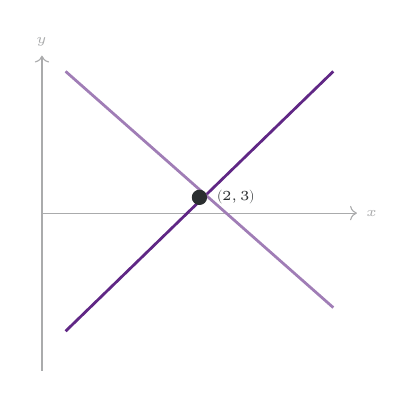
\begin{tikzpicture}[scale=1]
\draw[ink!40,->] (0,0) -- (40mm,0) node[right,font=\tiny] {$x$};
\draw[ink!40,->] (0,-20mm) -- (0,20mm) node[above,font=\tiny] {$y$};
\draw[accent,line width=1pt] (3mm,-15mm) -- (37mm,18mm);
\draw[accent!60,line width=1pt] (3mm,18mm) -- (37mm,-12mm);
\filldraw[ink] (20mm,2mm) circle (0.9mm);
\node[font=\sffamily\bfseries\tiny,text=ink,anchor=west] at (21mm,2mm) {$(2,3)$};
\end{tikzpicture}
\end{textblock*}

% ---- CARD 2: Substitution ----
\cardbg{16}{114}{178}{40}
\pill{26}{117}{Substitution method}

\begin{textblock*}{158mm}(26mm,130mm)
{\fontsize{11}{14}\selectfont\color{ink}
Isolate one variable, substitute into the other equation.}
\end{textblock*}

\begin{textblock*}{158mm}(26mm,141mm)
{\fontsize{13}{16}\selectfont $y=2x-1,\ 3x+y=9\ \Longrightarrow\ (x,y)=(2,3)$}
\end{textblock*}

% ---- CARD 3: Elimination ----
\cardbg{16}{160}{178}{40}
\pill{26}{163}{Elimination method}

\begin{textblock*}{158mm}(26mm,176mm)
{\fontsize{11}{14}\selectfont\color{ink}
Multiply so coefficients match, then add or subtract.}
\end{textblock*}

\begin{textblock*}{158mm}(26mm,187mm)
{\fontsize{13}{16}\selectfont $x+2y=11,\ 3x+y=18\ \Longrightarrow\ (x,y)=(5,3)$}
\end{textblock*}

\clearpage

% ======================================================================
% PAGE 2
% ======================================================================
\topicheader{2}{System of Equations}
\pagekicker{Rules sheet -- 2/2}
\pagefooter{13}
\mbox{}%

% ---- CARD 4: Special cases ----
\cardbg{16}{33}{178}{130}
\pill{26}{36}{Special cases}

\begin{textblock*}{158mm}(26mm,49mm)
{\fontsize{11}{14}\selectfont
\begin{tabular}{|p{54mm}|>{\centering\arraybackslash}p{91mm}|}
\hline
\rowcolor{accent}
{\color{white}\textbf{Coefficient ratios}} & {\color{white}\textbf{Result}} \\ \hline
Unequal & One solution \\ \hline
Equal, constants differ & No solution \\ \hline
Equal, constants equal & Infinitely many \\ \hline
\end{tabular}}
\end{textblock*}

\begin{textblock*}{50mm}(26mm,95mm)
{\centering\fontsize{10}{10}\selectfont\textbf{One solution}\par}
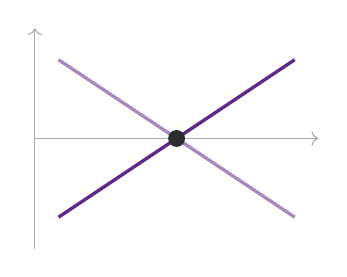
\begin{tikzpicture}
\draw[ink!40,->] (0,0) -- (36mm,0); \draw[ink!40,->] (0,-14mm) -- (0,14mm);
\draw[accent,line width=1.2pt] (3mm,-10mm) -- (33mm,10mm);
\draw[accent!55,line width=1.2pt] (3mm,10mm) -- (33mm,-10mm);
\filldraw[ink] (18mm,0) circle (1mm);
\end{tikzpicture}
\end{textblock*}

\begin{textblock*}{50mm}(82mm,95mm)
{\centering\fontsize{10}{10}\selectfont\textbf{No solution}\par}
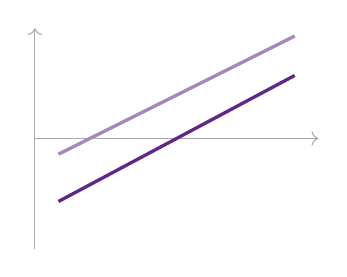
\begin{tikzpicture}
\draw[ink!40,->] (0,0) -- (36mm,0); \draw[ink!40,->] (0,-14mm) -- (0,14mm);
\draw[accent,line width=1.2pt] (3mm,-8mm) -- (33mm,8mm);
\draw[accent!55,line width=1.2pt] (3mm,-2mm) -- (33mm,13mm);
\end{tikzpicture}
\end{textblock*}

\begin{textblock*}{50mm}(138mm,95mm)
{\centering\fontsize{10}{10}\selectfont\textbf{Infinitely many}\par}
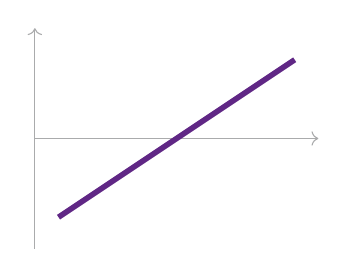
\begin{tikzpicture}
\draw[ink!40,->] (0,0) -- (36mm,0); \draw[ink!40,->] (0,-14mm) -- (0,14mm);
\draw[accent,line width=2pt] (3mm,-10mm) -- (33mm,10mm);
\end{tikzpicture}
\end{textblock*}

\end{document}
